% Homework template for Information Theory and Statistical Learning
% by Xiangxiang Xu <xiangxiangxu.thu@gmail.com>
% LAST UPDATE: Oct 3, 2019
\documentclass[a4paper]{article}
\usepackage[T1]{fontenc}
\usepackage{amsmath, amssymb, amsthm}
% amsmath: equation*, amssymb: mathbb, amsthm: proof
\usepackage{moreenum}
\usepackage{mathtools}
\usepackage{url}
\usepackage{enumitem}
\usepackage{bm}
\usepackage{graphicx}
\usepackage{subcaption}
\usepackage{booktabs} % toprule
\usepackage[mathcal]{eucal}
\usepackage{dsfont}
\usepackage[numbered,framed]{matlab-prettifier}
%% Definitions for Information Theory & Statistical Learning
%% UPDATED: Sep 30, 2019 by Xiangxiang 
\newcommand{\theterm}{Fall 2020}

\newcommand{\thecoursenameshort}{\textsc{Information Theory and Statistical Learning}}
\newcommand{\thecoursename}{
Tsinghua-Berkeley Shenzhen Institute\\
%\vspace*{0.1in}
\thecoursenameshort
}

\newcommand{\courseheader}{
\vspace*{-1in}
\begin{center}
\thecoursename \\
\theterm
\vspace*{0.1in}
\hrule
\end{center}
}
\newcommand{\uc}{\underline{c}}    % c, vec
\newcommand{\uv}{\underline{v}}    % x, vec
\newcommand{\uw}{\underline{w}}    % w, vec
\newcommand{\ux}{\underline{x}}    % x, vec
\newcommand{\uy}{\underline{y}}    % y, vec
\newcommand{\uz}{\underline{z}}    % z, vec
\newcommand{\um}{\underline{m}}    % m, vec
\newcommand{\ut}{\underline{t}}    % t, vec

\newcommand{\bA}{\mathbf{A}}    % A, mat
\newcommand{\bI}{\mathbf{I}}    % A, mat
\newcommand{\bN}{\mathbf{N}}    % n, mat
\newcommand{\bT}{\mathbf{T}}    % T, mat
\newcommand{\bU}{\mathbf{U}}    % U, mat
\newcommand{\bV}{\mathbf{V}}    % V, mat
\newcommand{\bQ}{\mathbf{Q}}    % Q, mat
\newcommand{\bX}{\mathbf{X}}    % X, mat

\newcommand{\bc}{\bm{c}}    % c, vec
\newcommand{\be}{\bm{e}}    % e, vec
\newcommand{\bu}{\bm{u}}    % u, vec
\newcommand{\bv}{\bm{v}}    % v, vec
\newcommand{\bw}{\bm{w}}    % w, vec
\newcommand{\bt}{\bm{t}}    % t, vec
\newcommand{\bx}{\bm{x}}    % x, vec
\newcommand{\by}{\bm{y}}    % y, vec
\newcommand{\bz}{\bm{z}}    % z, vec

\newcommand{\phib}{\bm{\phi}}    % phi, vec
\newcommand{\psib}{\bm{\psi}}    % psi, vec
\newcommand{\dtm}{\mathbf{B}}    %
\newcommand{\dtmt}{\tilde{\dtm}}    %
\newcommand{\Ab}{\mathbf{A}}    % A mat
\newcommand{\Kb}{\mathbf{K}}    % K mat
\newcommand{\Ib}{\mathbf{I}}    % I mat



\newcommand{\rvby}{\bm{\mathsf{y}}}    % y, rv. vec
\newcommand{\rvbx}{\bm{\mathsf{x}}}    % x, rv. vec
% \newcommand{\bm}{\bm{m}}    % m, vec
\newcommand{\bzero}{\bm{0}}    % 0, vec

\newcommand{\balpha}{\bm{\alpha}}    % alpha, vec
\newcommand{\bphi}{\bm{\phi}}    % phi, vec
\newcommand{\bpsi}{\bm{\psi}}    % psi, vec
\newcommand{\bxi}{\bm{\xi}}    % xi, vec
\newcommand{\btheta}{\bm{\theta}}    % theta, vec
\newcommand{\bmu}{\bm{\mu}}    % mu, vec

\newcommand{\bLambda}{\bm{\Lambda}}    % Sigma, mat
\newcommand{\bSigma}{\bm{\Sigma}}    % Sigma, mat

\newcommand{\cF}{\mathcal{F}}  
\newcommand{\cL}{\mathcal{L}}  
\newcommand{\cX}{\mathcal{X}}  
\newcommand{\cY}{\mathcal{Y}}  

\newcommand{\rvx}{\mathsf{x}}    % x, r.v.
\newcommand{\rvy}{\mathsf{y}}    % y, r.v.
\newcommand{\rvz}{\mathsf{z}}    % z, r.v.
\newcommand{\rvw}{\mathsf{w}}    % w, r.v.
\newcommand{\rvv}{\mathsf{v}}    % v, r.v.
\newcommand{\rvm}{\mathsf{m}}    % m, r.v.
\newcommand{\rvt}{\mathsf{t}}    % t, r.v.
\newcommand{\rvH}{\mathsf{H}}    % H, r.v.
\newcommand{\urvx}{\underline{\mathsf{x}}}    % x, r.v. vec
\newcommand{\urvy}{\underline{\mathsf{y}}}    % y, r.v. vec
\newcommand{\urvz}{\underline{\mathsf{z}}}    % z, r.v. vec
\newcommand{\urvw}{\underline{\mathsf{w}}}    % w, r.v. vec
\newcommand{\urvt}{\underline{\mathsf{t}}}    % t, r.v. vec


\newcommand{\defeq}{\triangleq} %\coloneqq
\newcommand{\reals}{\mathbb{R}}
\newcommand{\T}{\mathrm{T}}    % transpose
\newcommand{\F}{\mathrm{F}}    % Frobenius
\newcommand{\BLS}{\mathrm{BLS}}    % BLS
\newcommand{\LLS}{\mathrm{LLS}}    % LLS
\newcommand{\MVU}{\mathrm{MVU}}    % MVU
\newcommand{\dd}{\mathrm{d}}  

\DeclareMathOperator*{\maximize}{maximize}    % maximize
\DeclareMathOperator*{\minimize}{minimize}    % minimize
\newcommand{\st}{\mathrm{subject~to}}    % minimize

% \newcommand{\E}[1]{\mathbb{E}\left[{#1}\right]}
% \newcommand{\Prob}[1]{\mathbb{P}\left({#1}\right)}
\DeclareMathOperator*{\argmax}{arg\,max}
\DeclareMathOperator*{\argmin}{arg\,min}
\DeclareMathOperator*{\argsup}{arg\,sup}
\DeclareMathOperator*{\arginf}{arg\,inf}
\DeclareMathOperator{\diag}{diag}
\DeclareMathOperator{\tr}{tr}
\DeclareMathOperator{\Cov}{Cov}
\DeclareMathOperator{\var}{var}
\DeclareMathOperator{\cov}{cov}
\DeclareMathOperator{\MSE}{MSE}
\DeclareMathOperator{\1}{\mathds{1}} % dsfont required
\DeclareMathOperator{\E}{\mathbb{E}}
\DeclareMathOperator{\Prob}{\mathbb{P}}
\DeclareMathOperator{\im}{im}
\DeclareMathOperator{\rank}{rank}
\DeclareMathOperator{\Bern}{Bern}
\DeclareMathOperator{\Binom}{Binom}

\newcommand\independent{\protect\mathpalette{\protect\independenT}{\perp}}
\def\independenT#1#2{\mathrel{\rlap{$#1#2$}\mkern2mu{#1#2}}}

%%% Local Variables:
%%% mode: latex
%%% TeX-master: "ithw"
%%% End:


\lstset{
  style              = Matlab-editor,
  captionpos         =b,
  basicstyle         = \mlttfamily,
  escapechar         = ",
  mlshowsectionrules = true,
}
\begin{document}
\courseheader



\newcounter{hwcnt}
\setcounter{hwcnt}{1} % set to the times of Homework

\begin{center}
  \underline{\bf Homework \thehwcnt} \\
\end{center}
\begin{flushleft}
  \textcolor{gray}{YOUR NAME}\hfill
  \today
\end{flushleft}
\hrule

\vspace{2em}
\setlist[enumerate,1]{label=\thehwcnt.\arabic*.}
\setlist[enumerate,2]{label=(\alph*)}
\setlist[enumerate,3]{label=\roman*.}
\setlist[enumerate,4]{label=\greek*)}

\flushleft
\rule{\textwidth}{1pt}
\begin{itemize}
\item {\bf Acknowledgments: \/} 
  \textcolor{gray}{This template takes some materials from course CSE 547/Stat 548 of Washington University: \small{\url{https://courses.cs.washington.edu/courses/cse547/17sp/index.html}}.}

  \textcolor{red}{If you refer to other materials in your homework, please list here.}
\item {\bf Collaborators: \/}
  \textcolor{gray}{I finish this template by myself.} \textcolor{red}{If you finish your homework all by yourself, make a similar statement. If you get help from others in finishing your homework, state like this:}
  \textcolor{gray}{
  \begin{itemize}
  \item 1.2 (b) was solved with the help from \underline{\hspace{3em}}.
  \item Discussion with \underline{\hspace{3em}} helped me finishing 1.3.
  \end{itemize}
}
\item  \emph{I certify that all solutions are entirely in my words and that I have not looked at another student's solutions. I have credited all external sources in this write up.}
  \framebox[\linewidth]{\rule{0pt}{10pt}\textcolor{gray}{\large Your signature}}
\end{itemize}
\rule{\textwidth}{1pt}


\vspace{2em}

You may use \texttt{enumerate} to generate answers for each question:

\begin{enumerate}
  \setlength{\itemsep}{3\parskip}

\item You may find \url{https://en.wikibooks.org/wiki/LaTeX} useful.
  \begin{enumerate}
    \item Writing \LaTeX\ online may be easier for beginners. You may find Overleaf (\url{https://www.overleaf.com/}) useful.
    \end{enumerate}
  \item You may need aligned equations for your homework, here are several examples:
    
    Total probability rule:
  \begin{equation*}
    \begin{aligned}
      \Prob(X = x)
      &= \sum_{y \in \mathcal{Y}} \Prob(X = x, Y = y)\\
      &= \sum_{y \in \mathcal{Y}} \Prob(X = x| Y = y) \Prob(Y = y),\\
    \end{aligned}
  \end{equation*}
  or
  \begin{equation*}
    \begin{aligned}
      P_{X}(x)
      &= \sum_{y \in \mathcal{Y}} P_{XY}(x,y)\\
      &= \sum_{y \in \mathcal{Y}} P_{X|Y}(x|y)P_{Y}(y).\\
    \end{aligned}
  \end{equation*}
  Indicator function:
  \begin{equation*}
    \1_A(\omega)=
    \left\{
    \begin{aligned}
      1, &\quad\text{if}~ \omega \in A,\\
      0, &\quad\text{if}~ \omega \notin A.
    \end{aligned}
    \right.
  \end{equation*}

  \item You may need to add figures and source codes in your homework. Figure \ref{fig:1} is an example that compares the empirical distribution (histogram) and probability density function of a Gaussian random variable.
    \begin{figure}[htbp]
      \centering
      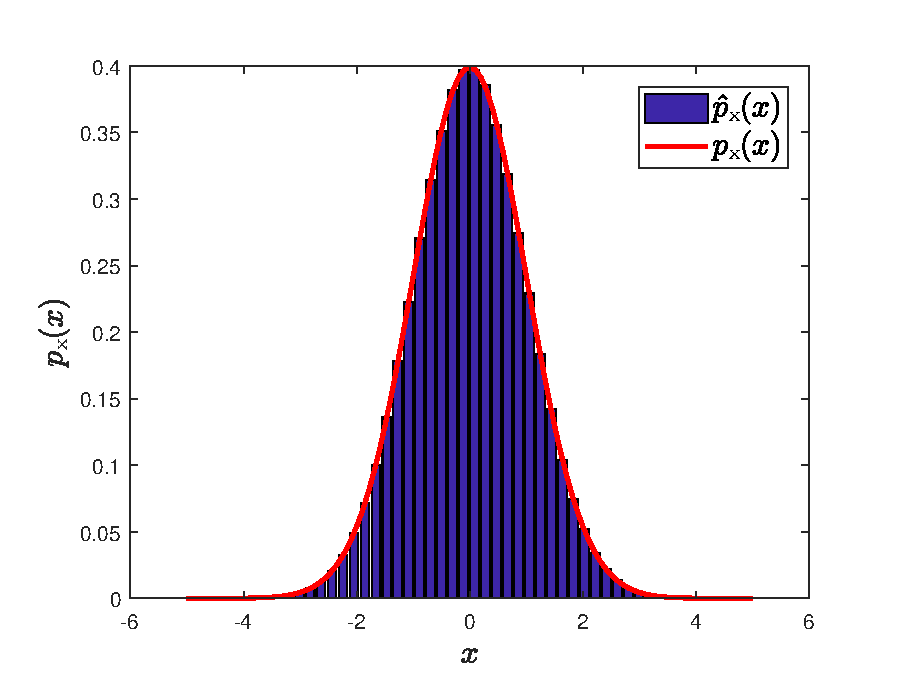
\includegraphics[width = 0.8\textwidth]{pdf_normal.eps}
      \caption{Gaussian PDF and histogram of samples}
      \label{fig:1}
    \end{figure}

  The source code to plot Figure \ref{fig:1} could be found in Appendix \ref{sec:a:code}. Here are the core codes:
  \lstinputlisting[firstline=4,lastline=4, firstnumber=4]{matlabscript.m}
  \lstinputlisting[firstline=6,lastline=7, firstnumber=6]{matlabscript.m}
  To understand line 6, note that if we have $n$ samples of $X$ denoted by $x^{(i)}, i = 1, 2, \cdots, n$, then the probability density function $p_{X}$ can be estimated as
  \begin{equation*}
    \begin{aligned}
      p_{X}(x_0) &= \left.\frac{\mathrm{d}}{\mathrm{d}x} \Prob(X \leq x) \right|_{x = x_0} \\
      &\approx \frac{\Prob(x_0 - \Delta x < X \leq x_0)}{\Delta x}\\
      &\approx \frac{1}{n\Delta x} \sum_{i = 1}^n \1_{x^{(i)} \in (x_0 - \Delta x, x_0]}.
    \end{aligned}    
  \end{equation*}
    
\end{enumerate}
  
  \newpage
  
  \appendix
  \section{Source code}
  \label{sec:a:code}
  % \lstlistoflistings
  The source code for plotting Figure \ref{fig:1} is shown as follows.
  \lstinputlisting{matlabscript.m}
  
\end{document}
%%% Local Variables:
%%% mode: latex
%%% TeX-master: t
%%% End:
